\section{Fourier-Polynome und Projektion (+)}\label{MA2-fourierpolynome-und-projektion}

\begin{table}[H]
  \centering
  \begin{tabularx}{\textwidth}{@{}>{\raggedright\arraybackslash}X r@{}}
    \toprule
    \multicolumn{2}{c}{\textbf{�bersicht �ber Lernziele und Voraussetzungen}}\\
    \midrule
    \textbf{Lernziele} & \\[.5\normalbaselineskip]
    \tabitem ein Fourier-Polynom als Element eines endlichdimensionalen Unterraums interpretieren & \\
    \tabitem den Approximationsraum $U_N$ explizit beschreiben & \\
    \tabitem das Fourier-Polynom als orthogonale Projektion einer Funktion auf $U_N$ verstehen & \\
    \tabitem die Bestapproximationseigenschaft mit Hilfe des Skalarprodukts formulieren & \\
    \tabitem das Residuum als orthogonalen Fehler interpretieren & \\[.5\normalbaselineskip]
    \midrule
    \textbf{Voraussetzungen} & \\[.5\normalbaselineskip]
    \tabitem mit Orthonormalsystemen in Funktionenr�umen umgehen k�nnen & \abschnittsverweis{MA2-integrierbare-funktionen}\\
    \tabitem Skalarprodukt und Norm in Funktionenr�umen anwenden k�nnen & \abschnittsverweis{MA2-integrierbare-funktionen} \\
    \tabitem Fourier-Koeffizienten berechnen k�nnen & \abschnittsverweis{MA2-fourierreihen}  \\
    \bottomrule
  \end{tabularx}
\end{table}

\noindent \ifintegriereaufgaben Die �bungsaufgaben zum Thema finden Sie \hyperref[MA2-fourierpolynome-und-projektion-aufgaben]{hier}.
\vspace{0.3cm}
\hrule
\fi

Die Fourier-Reihe wurde als Entwicklung einer Funktion in einem Orthonormalsystem mit unendlich vielen Basisfunktionen eingef�hrt.

Liegt ein global stetiges, $T$-periodisches Signal $u$ vor, so konvergiert die Fourier-Reihe punktweise gegen $f$:

\[
u(t)
=
\frac{a_0}{2}
+
\sum_{n=1}^{\infty}
\left(
	a_n\cdot \cos(\omega_n\, t)
+
b_n \cdot \sin(\omega_n\, t)
\right)\,, \quad \omega_n = n\cdot \omega_0\,.
\]

\bigskip

\subsection*{Abbruch nach endlich vielen Harmonischen}

Bricht man die Reihenentwicklung nach $N$ Harmonischen ab, so erh�lt man ein Fourier-Polynom vom Grad $N$:

\[
u_N(t)
=
\frac{a_0}{2}
+
\sum\limits_{n=1}^{N}
\left(
	a_n \cdot \cos(\omega_n\, t)
+
b_n \cdot \sin(\omega_n\, t)
\right)\,, \quad \omega_n = n\cdot \omega_0\,.
\]

Im Allgemeinen gilt:
\[
	u_N \neq u\,.
\]

Was also ist $u_N$?  Welche Bedeutung besitzt dieses Polynom?

\subsection*{Der zugrunde liegende Unterraum}

Betrachten wir den endlichdimensionalen Raum

\[
U_N
=
\mathrm{LH}
\left\{
	1,\cos(\omega_0\, t),\sin(\omega_0\, t),\cos(\omega_1\, t),\sin(\omega_1\, t),\cos(\omega_2\, t),\sin(\omega_2\, t),
\dots,
\cos(\omega_N\, t),\sin(\omega_N\, t)
\right\} \,..
\]

Dieser Raum enth�lt die - \textbf{und nur die} - Fourier-Polynome vom Grad $N$. Er ist ein Unterraum des Funktionenraums der $T$-periodischen Funktionen. Das Fourier-Polynom $u_N$ ist ein Element dieses Raumes.

\subsection*{Beste Approximation}

Unter allen Funktionen $q \in U_N$ ist $u_N$ ausgezeichnet durch die Eigenschaft:

\[
\|u - u_N\|
=
\min_{q \in U_N}
\|u - q\|.
\]

In Worten: \(u_N\) besitzt den k�rzesten Abstand zu \(u\)! Wir sagen auch \(u_N\) ist die Bestapproximation von $u$ im Raum $U_N$ - ganz pr�zise die Bestapproximation von $u$ bez�glich der durch das Skalarprodukt induzierten Norm. Die folgende Skizze veranschaulicht die Eigenschaft von \(u_N\):
\bigskip
 \begin{center}
	 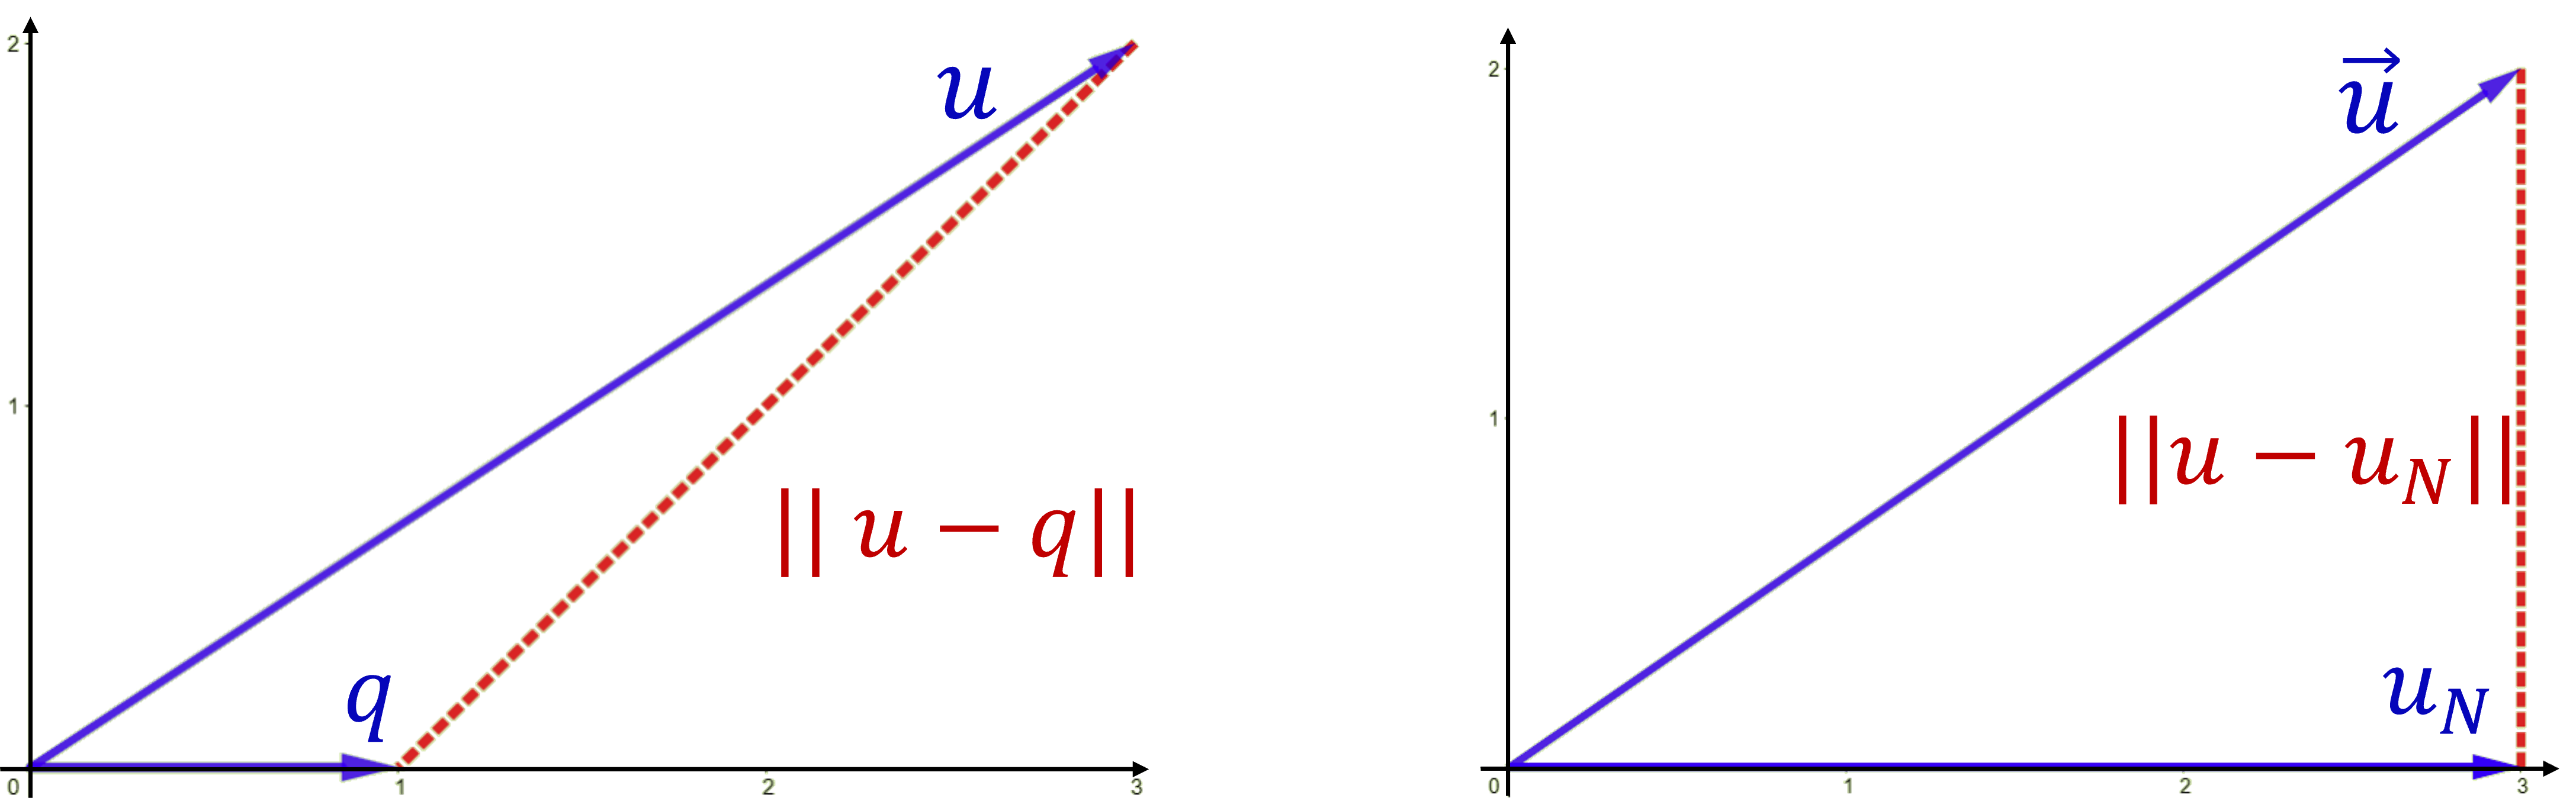
\includegraphics[width=0.7\textwidth]{../Mathematik_2/Bilder/bestapproximation_abstandsminimum_gerade.png}
 \end{center}

\subsection*{Das Residuum}

Definieren wir das sogenannte Residuum (den Abstand zwischen \(u\) und der Bestapproximation)

\[
	r := u - u_N\,.
\]

Minimal ist das Residuum genau dann, wenn es orthogonal auf dem gesamten Raum $U_N$ steht:

\[
\langle r , q \rangle = 0
\quad \text{f�r alle } q \in U_N.
\]

Insbesondere gilt f�r alle \(n \leq N\):

\[
\langle u - u_N , \hat c_n \rangle = 0,
\qquad
\langle u - u_N , \hat s_n \rangle = 0.
\]

\medskip

Das Residuum enth�lt also keine Anteile mehr in Richtung der harmonischen Schwingungen bis zur Ordnung $N$:
\[
\text{Fehler} \perp \text{Approximationsraum}.
\]

Das Fourier-Polynom $u_N$ ist die beste Approximation an die Funktion $u$ auf den Unterraum $U_N$; jedes andere Element des Raumes $U_N$ besitzt einen gr��eren Abstand zu $u$.
